\documentclass{article}
\usepackage{amsmath}
\usepackage{graphicx}

\title{Assignment3}
\author{Teja Vardhan Shannu}
\date{August 2024}

\begin{document}
\maketitle
\textbf{Problem:} A line intersects the Y-axis and the X-axis at the points $P(0,b)$ and $Q(c,0)$ respectively. If $(2,-5)$ is the midpoint of $PQ$, then find the coordinates of $P$ and $Q$.

\begin{table}[h]
\centering

\begin{tabular}{|c|c|}
\hline
Input & Output\\ \hline
P & {P} = $\begin{pmatrix} 0 \\ b \end{pmatrix}$\\ \hline
Q & {Q} = $\begin{pmatrix} c \\ 0 \end{pmatrix}$ \\ \hline
M & {M} = $\begin{pmatrix} 2 \\ -5 \end{pmatrix}$ \\ \hline

\end{tabular}
\end{table}

\textbf{Solution:}




Let the coordinates of points $P$ and $Q$ be represented by the vectors:
\[
\mathbf{P} = \begin{pmatrix} 0 \\ b \end{pmatrix}, \quad \mathbf{Q} = \begin{pmatrix} c \\ 0 \end{pmatrix}
\]
The midpoint $M$ is given as:
\[
\mathbf{M} = \begin{pmatrix} 2 \\ -5 \end{pmatrix}
\]
The midpoint formula in vector form is:
\[
\mathbf{M} = \frac{1}{2} (\mathbf{P} + \mathbf{Q})
\]
Substituting the given values:
\[
\frac{1}{2} \left(\begin{pmatrix} 0 \\ b \end{pmatrix} + \begin{pmatrix} c \\ 0 \end{pmatrix}\right) = \begin{pmatrix} 2 \\ -5 \end{pmatrix}
\]
This simplifies to:
\[
\frac{1}{2} \begin{pmatrix} c \\ b \end{pmatrix} = \begin{pmatrix} 2 \\ -5 \end{pmatrix}
\]
Multiplying both sides by 2:
\[
\begin{pmatrix} c \\ b \end{pmatrix} = \begin{pmatrix} 4 \\ -10 \end{pmatrix}
\]
Thus, the coordinates of $P$ and $Q$ are:
\[
\mathbf{P} = \begin{pmatrix} 0 \\ -10 \end{pmatrix}, \quad \mathbf{Q} = \begin{pmatrix} 4 \\ 0 \end{pmatrix}
\]

\begin{figure}[h!]
  \hspace{0cm}
  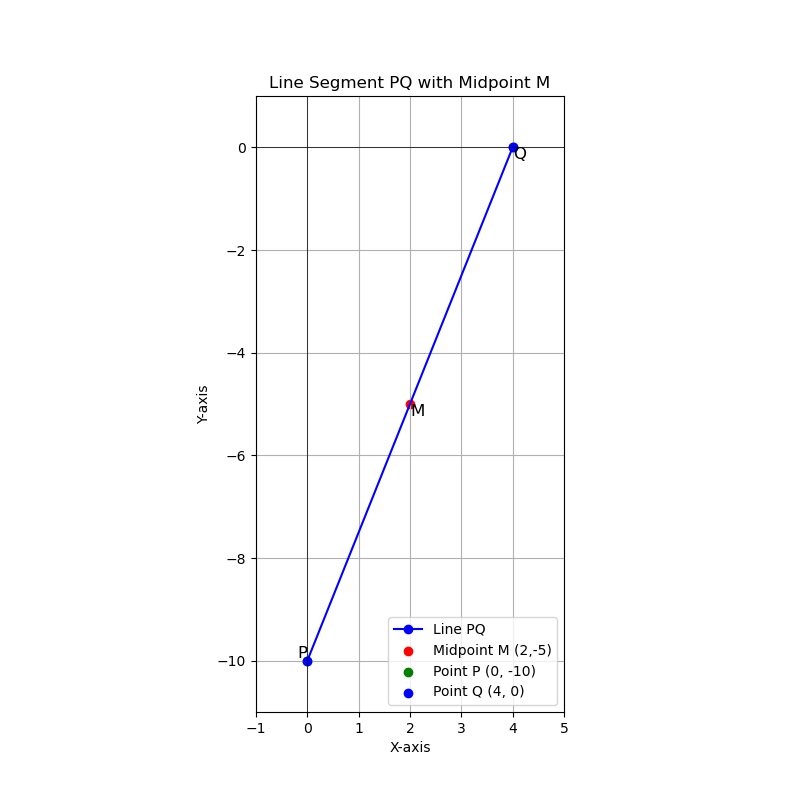
\includegraphics[width=1.0\textwidth]{Figure_1.png}
  
  \caption{The plot of the points }
  \label{fig:your_label}
\end{figure}


\end{document}

